\usetikzlibrary{calc,arrows.meta,patterns,angles,quotes}
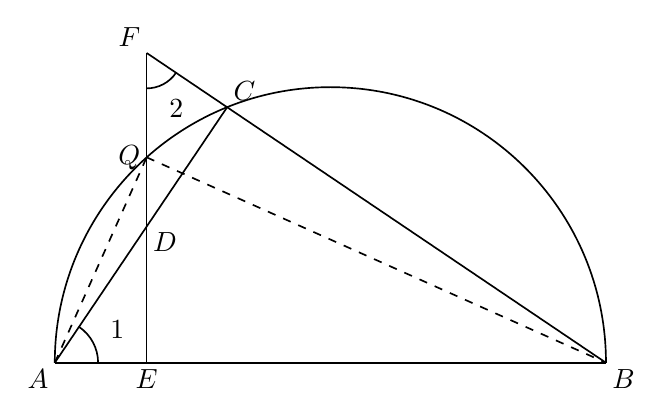
\begin{tikzpicture}[x=1cm,y=1cm,line width=.6pt,font=\normalsize,>=Stealth]
\coordinate (O) at (0.0000000000,0.0000000000);
\coordinate (A) at (-3.5000000000,0.0000000000);
\coordinate (B) at (3.5000000000,0.0000000000);
\coordinate (C) at (-1.3111230770,3.2451434910);
\coordinate (E) at (-2.3333333333,0.0000000000);
\coordinate (D) at (-2.3333333333,1.7296544633);
\coordinate (F) at (-2.3333333333,3.9346330149);
\coordinate (Q) at (-2.3333333333,2.6087459737);
\draw (3.5000000000,0.0000000000) arc[start angle=0.0000000000,end angle=180.0000000000,radius=3.5000000000cm];
\draw (A)--(B);
\draw (E)--(F);
\draw (A)--(C);
\draw (F)--(B);
\draw[dashed] (A)--(Q);
\draw[dashed] (Q)--(B);
\draw (-2.9500000000,0.0000000000) arc[start angle=0.0000000000,end angle=56.0000000000,radius=0.5500000000cm];
\draw (-2.3333333333,3.4846330149) arc[start angle=270.0000000000,end angle=326.0000000000,radius=0.4500000000cm];
\node[below left=2pt,inner sep=0pt] at (A) {$A$};
\node[below right=2pt,inner sep=0pt] at (B) {$B$};
\node[above right=2pt,inner sep=0pt] at (C) {$C$};
\node[below=2pt,inner sep=0pt] at (E) {$E$};
\node[below right=2pt,inner sep=0pt] at (D) {$D$};
\node[above left=2pt,inner sep=0pt] at (F) {$F$};
\node[left=2pt,inner sep=0pt] at (Q) {$Q$};
\node at (-2.7053471664,0.4225244065) {$1$};
\node at (-1.9577560831,3.2282749406) {$2$};
\end{tikzpicture}
